% Drawing 154/07-25 -- folder 154, batch 07, archive page 140 (PDF page 141).
% Transcription: grand dessin au crayon et à l'encre, sans texte : un faisceau de pseudo-droites étiquetées de lettres $A, \ldots, G$ et de numéros entourés $1, 1', 2, \ldots, 11$, dont les points d'intersection sont nommés $a_0, a_1, \ldots, a_{10}$, $b_1, b_2, \ldots, b_{10}$ (avec « $b_{-1} = b_{10}$ » en haut), $c_1, c_{11}$, $d_1, d_{11}$, $e_1, e_{10}, e_{11}$, $f_1, f_{11}$, $g_1, g_{11}$ ; des bandes hachurées et en tirets suivent les pseudo-droites, et trois triangles sont noircis. À droite, un quadrillage de droites $A, \ldots, G$ (verticales) et $1, \ldots, 5$ (horizontales), avec des diagonales tracées sur les colonnes $D$ à $G$ ; au-dessus, une double ligne fléchée numérotée $1$, $2$ ; et deux petits croquis de droites qui se coupent
% Kind: whole-page arrangement A..G with a sweep numbered 1..11; grid A..G by 1..5. Method 2 (schematic redraw from the facsimile). Status: partial.
% Notes: Whole-page figure, redrawn as a skeleton. Drawn: the pseudo-lines A and F (straight, crossing in the upper left), the curved lines through d_1 and c_1 (the two arcs of C and D as read), the vertical line 11 with d_11, c_11, g_11, f_11, e_11 on it, the lines 1 and 1' of the sweep (from the lower left through d_1, e_1, f_1, g_1 and the knot of the a's to c_1 and the upper right), and the outer line 8 of the sweep; the named points with their letters, placed as on the page; the circled numbers at both ends of the sweep; the grid at the right with its letters, numbers and three diagonals; the double arrowed line 1, 2 above it; the two small sketches of crossing lines. Not drawn: the intermediate lines 2 to 7 and 9, 10 of the sweep, all hatched and dashed bands, the three blackened triangles, and the dotted line towards the circled 9. Which letter belongs to which curved line is read from the labels at the ends (E, D, C at the bottom, D, E, B, G at the top) and is not sure for C and D. Redrawn 2026-11-12 (issue 128): to check again.
% Coordinates: 1 unit = 1 mm = 1/100 of the crop width (bbox in page fractions: [0.1, 0.065, 0.97, 0.55]).
% Redrawn by Claude (claude-fable-5-2), issue #128, 2026-11-12; not checked by a human; not compiled (no TeX in the session).
% Rights: reproduces part of the work -- behind RENDER_TRANSCRIPTS, never published by itself.
\documentclass[tikz,border=3pt]{standalone}
\usepackage{amsmath,amssymb}
\usetikzlibrary{patterns,arrows.meta}
\tikzset{pencil/.style={black!45}, struck/.style={black!35}, mpt/.style={circle,draw,inner sep=1.3pt}, pt/.style={circle,fill,inner sep=0.9pt}, opt/.style={circle,draw,fill=white,inner sep=1.1pt}}
\begin{document}
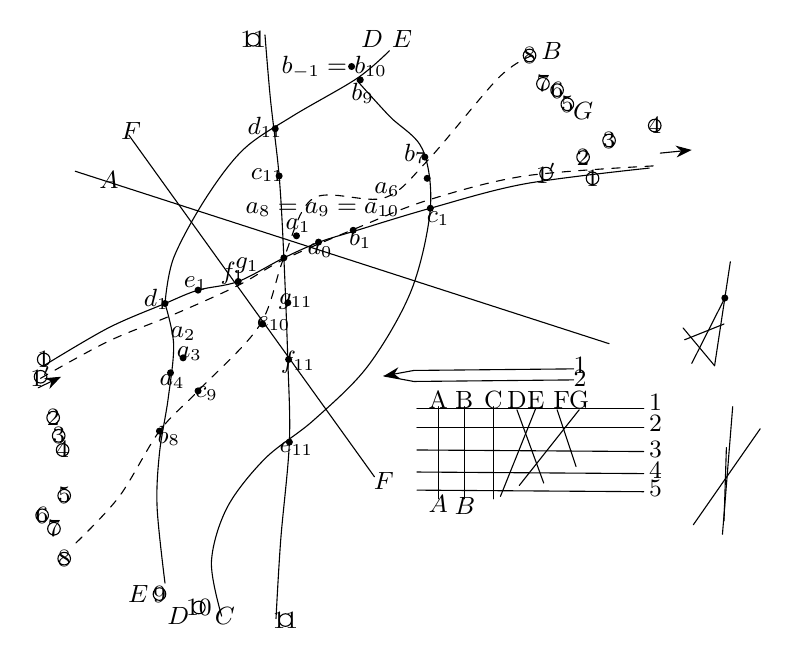
\begin{tikzpicture}[x=1mm,y=1mm,line cap=round,line join=round,font=\scriptsize]
\draw (7,-18.6) -- (74.8,-40.5);
\node[inner sep=1pt] at (11.3,-19.7) {\small $A$};
\draw (13.8,-14) -- (45,-57.4);
\node[inner sep=1pt] at (14.1,-13.5) {\small $F$};
\node[inner sep=1pt] at (46.2,-58) {\small $F$};
\draw plot[smooth, tension=0.55] coordinates {(31.1,-1.3) (31.8,-9.5) (32.9,-19.2) (33.5,-29.6) (34,-42.6) (34.2,-53) (33.1,-65.4) (32.5,-75.4)};
\draw (29.6,-1.9) circle[radius=0.8];
\node[inner sep=1pt] at (29.6,-1.9) {\small 11};
\draw (33.7,-75.6) circle[radius=0.8];
\node[inner sep=1pt] at (33.7,-75.6) {\small 11};
\draw plot[smooth, tension=0.55] coordinates {(18.4,-35.4) (19.5,-29.6) (23.6,-22) (28.4,-15.8) (34.6,-11.6) (42.8,-6.8) (46.9,-3.3)};
\draw plot[smooth, tension=0.55] coordinates {(18.4,-35.4) (19.5,-40.6) (18.8,-47.5) (17.7,-54.4) (17.4,-61.3) (18.4,-70.9)};
\draw plot[smooth, tension=0.55] coordinates {(42.8,-7.1) (46.9,-11.6) (51.1,-15.8) (52.1,-23.3) (49.7,-33.7) (44.2,-43.3) (37.3,-50.2) (31.1,-55.1) (26.3,-61.3) (24.3,-68.2) (25.6,-75.1)};
\draw plot[smooth, tension=0.55] coordinates {(3,-43.3) (11.2,-38.5) (18.4,-35.4) (22.6,-33.7) (27.7,-32.6) (33.5,-29.6) (38,-27.6) (42.8,-26.1) (52.1,-23.3) (64.1,-20.2) (79.9,-18.2)};
\draw[dashed] plot[smooth, tension=0.55] coordinates {(2.6,-44.9) (11.2,-40.2) (19.5,-36.8) (27.7,-33.1) (33.5,-29.8) (42.8,-25.8) (51.7,-22.3) (64.1,-19.2) (80.9,-17.9)};
\draw[dashed] plot[smooth, tension=0.55] coordinates {(7.1,-65.8) (12.6,-59.9) (17.7,-51.6) (22.6,-46.5) (30.4,-38.2) (33.5,-29.6) (37.3,-22) (46.2,-22) (51.7,-17.3) (60.7,-6.8) (64.8,-4)};
\node[pt] at (18.4,-35.4) {};
\node[pt] at (22.6,-33.7) {};
\node[pt] at (27.7,-32.6) {};
\node[pt] at (33.5,-29.6) {};
\node[pt] at (52.1,-23.3) {};
\node[pt] at (51.7,-19.5) {};
\node[pt] at (51.4,-16.8) {};
\node[pt] at (42.1,-5.3) {};
\node[pt] at (43.2,-7) {};
\node[pt] at (32.4,-13.2) {};
\node[pt] at (32.9,-19.2) {};
\node[pt] at (34,-35.3) {};
\node[pt] at (34.1,-42.5) {};
\node[pt] at (34.2,-53) {};
\node[pt] at (30.8,-38) {};
\node[pt] at (22.6,-46.5) {};
\node[pt] at (17.7,-51.6) {};
\node[pt] at (20.7,-42.3) {};
\node[pt] at (19.1,-44.2) {};
\node[pt] at (37.9,-27.6) {};
\node[pt] at (42.3,-26.1) {};
\node[pt] at (35.1,-26.8) {};
\node[inner sep=1pt] at (17.3,-34.9) {\small $d_1$};
\node[inner sep=1pt] at (22.3,-32.9) {\small $e_1$};
\node[inner sep=1pt] at (27,-31.5) {\small $f_1$};
\node[inner sep=1pt] at (28.8,-30.6) {\small $g_1$};
\node[inner sep=1pt] at (53.1,-24.6) {\small $c_1$};
\node[inner sep=1pt] at (39.9,-5.4) {\small $b_{-1}=b_{10}$};
\node[inner sep=1pt] at (43.5,-8.7) {\small $b_9$};
\node[inner sep=1pt] at (31.1,-13) {\small $d_{11}$};
\node[inner sep=1pt] at (31.4,-19.1) {\small $c_{11}$};
\node[inner sep=1pt] at (35,-35.2) {\small $g_{11}$};
\node[inner sep=1pt] at (35.3,-42.8) {\small $f_{11}$};
\node[inner sep=1pt] at (35.1,-53.8) {\small $e_{11}$};
\node[inner sep=1pt] at (32.2,-38) {\small $e_{10}$};
\node[inner sep=1pt] at (23.7,-46.8) {\small $c_9$};
\node[inner sep=1pt] at (18.9,-52.2) {\small $b_8$};
\node[inner sep=1pt] at (38.1,-28.7) {\small $a_0$};
\node[inner sep=1pt] at (43.2,-27.1) {\small $b_1$};
\node[inner sep=1pt] at (35.3,-25.5) {\small $a_1$};
\node[inner sep=1pt] at (20.7,-39.2) {\small $a_2$};
\node[inner sep=1pt] at (21.5,-41.8) {\small $a_3$};
\node[inner sep=1pt] at (19.3,-45.3) {\small $a_4$};
\node[inner sep=1pt] at (46.6,-20.9) {\small $a_6$};
\node[inner sep=1pt] at (38.4,-23.5) {\small $a_8=a_9=a_{10}$};
\node[inner sep=1pt] at (50.2,-16.4) {\small $b_7$};
\node[inner sep=1pt] at (67.5,-3.3) {\small $B$};
\node[inner sep=1pt] at (71.5,-10.9) {\small $G$};
\node[inner sep=1pt] at (15,-72.3) {\small $E$};
\node[inner sep=1pt] at (20.1,-75.1) {\small $D$};
\node[inner sep=1pt] at (26,-75.1) {\small $C$};
\node[inner sep=1pt] at (44.7,-1.8) {\small $D$};
\node[inner sep=1pt] at (48.5,-1.8) {\small $E$};
\draw (3,-42.5) circle[radius=0.8];
\node[inner sep=1pt] at (3,-42.5) {\small 1};
\draw (2.6,-44.7) circle[radius=0.8];
\node[inner sep=1pt] at (2.6,-44.7) {\small $1'$};
\draw (4.2,-49.9) circle[radius=0.8];
\node[inner sep=1pt] at (4.2,-49.9) {\small 2};
\draw (4.9,-52.2) circle[radius=0.8];
\node[inner sep=1pt] at (4.9,-52.2) {\small 3};
\draw (5.4,-54) circle[radius=0.8];
\node[inner sep=1pt] at (5.4,-54) {\small 4};
\draw (5.6,-59.8) circle[radius=0.8];
\node[inner sep=1pt] at (5.6,-59.8) {\small 5};
\draw (2.8,-62.3) circle[radius=0.8];
\node[inner sep=1pt] at (2.8,-62.3) {\small 6};
\draw (4.3,-64) circle[radius=0.8];
\node[inner sep=1pt] at (4.3,-64) {\small 7};
\draw (5.6,-67.8) circle[radius=0.8];
\node[inner sep=1pt] at (5.6,-67.8) {\small 8};
\draw (17.7,-72.3) circle[radius=0.8];
\node[inner sep=1pt] at (17.7,-72.3) {\small 9};
\draw (22.7,-74) circle[radius=0.8];
\node[inner sep=1pt] at (22.7,-74) {\small 10};
\draw (72.7,-19.5) circle[radius=0.8];
\node[inner sep=1pt] at (72.7,-19.5) {\small 1};
\draw (66.8,-18.9) circle[radius=0.8];
\node[inner sep=1pt] at (66.8,-18.9) {\small $1'$};
\draw (71.5,-16.8) circle[radius=0.8];
\node[inner sep=1pt] at (71.5,-16.8) {\small 2};
\draw (74.8,-14.7) circle[radius=0.8];
\node[inner sep=1pt] at (74.8,-14.7) {\small 3};
\draw (80.6,-12.8) circle[radius=0.8];
\node[inner sep=1pt] at (80.6,-12.8) {\small 4};
\draw (69.5,-10.1) circle[radius=0.8];
\node[inner sep=1pt] at (69.5,-10.1) {\small 5};
\draw (68.2,-8.3) circle[radius=0.8];
\node[inner sep=1pt] at (68.2,-8.3) {\small 6};
\draw (66.4,-7.5) circle[radius=0.8];
\node[inner sep=1pt] at (66.4,-7.5) {\small 7};
\draw (64.7,-3.9) circle[radius=0.8];
\node[inner sep=1pt] at (64.7,-3.9) {\small 8};
\draw[-{Stealth[length=2mm]}] (81.3,-16.3) -- (85.3,-15.9);
\draw[-{Stealth[length=2mm]}] (2.3,-46.1) -- (5.2,-44.7);
\draw (53.1,-48.5) -- (53.1,-60.2);
\draw (56.4,-48.5) -- (56.4,-60.2);
\draw (60.1,-48.5) -- (60.1,-60.2);
\draw (50.4,-48.7) -- (79.2,-48.7);
\draw (50.4,-51.1) -- (79.2,-51.1);
\draw (50.4,-54) -- (79.2,-54.2);
\draw (50.4,-56.8) -- (79.2,-57);
\draw (50.4,-59.1) -- (79.2,-59.3);
\draw (63.1,-48.9) -- (66.5,-58.2);
\draw (65.5,-48.7) -- (61,-59.9);
\draw (68.2,-48.9) -- (70.6,-56.1);
\draw (71,-48.9) -- (63.4,-58.5);
\node[inner sep=1pt] at (53.1,-47.7) {\small A};
\node[inner sep=1pt] at (56.4,-47.7) {\small B};
\node[inner sep=1pt] at (60.1,-47.7) {\small C};
\node[inner sep=1pt] at (63.1,-47.7) {\small D};
\node[inner sep=1pt] at (65.5,-47.7) {\small E};
\node[inner sep=1pt] at (68.8,-47.7) {\small F};
\node[inner sep=1pt] at (71,-47.7) {\small G};
\node[inner sep=1pt] at (53.1,-60.9) {\small $A$};
\node[inner sep=1pt] at (56.5,-61.1) {\small $B$};
\node[inner sep=1pt] at (80.7,-48) {\small 1};
\node[inner sep=1pt] at (80.7,-50.6) {\small 2};
\node[inner sep=1pt] at (80.7,-54) {\small 3};
\node[inner sep=1pt] at (80.7,-56.6) {\small 4};
\node[inner sep=1pt] at (80.7,-58.9) {\small 5};
\draw[{Stealth[length=2mm]}-] (46.2,-44.6) -- (50,-43.9) -- (70.3,-43.7);
\draw (46.2,-44.6) -- (50,-45.3) -- (70.3,-45.1);
\node[inner sep=1pt] at (71.1,-43.3) {\small 1};
\node[inner sep=1pt] at (71.1,-44.9) {\small 2};
\draw (90.2,-30.1) -- (88.2,-43.3);
\draw (89.5,-34.7) -- (85.3,-43);
\draw (84.2,-38.5) -- (88.2,-43.3);
\draw (84.4,-40) -- (89.4,-38);
\node[pt] at (89.5,-34.7) {};
\draw (90.5,-48.5) -- (89.2,-64.7);
\draw (94,-51.3) -- (85.5,-63.5);
\draw (89.7,-53.7) -- (89.4,-63);
\end{tikzpicture}
\end{document}
